\section{A sharp uniform Euler bound at every positive real order}
\label{sec:euler}

The canonical manuscript proves one-sided Euler enclosures in several
parameter regions. It also proves that the Gaussian magnitude has a unique
global maximum on the outer-order axis. It explicitly cautions that a
magnitude bound alone is not a remainder bound in the supercritical
region. The missing implication is supplied here by a sharp, elementary
two-point inequality. No finite signed-moment representation is needed.

\subsection{Definitions and the exact two-measure representation}

For $a\geq0$, $b>0$, let
\[
 H_m^{(b)}=\sum_{j=1}^m j^{-b},\qquad
 F_{a,b}(z)=\sum_{n\geq1}\frac{H_{n-1}^{(b)}}{n^a}z^n,
 \qquad |z|<1.
\]
For integral positive orders this is the decreasing-index multiple
polylogarithm $\Li_{a,b}(z,1)$. Write
$g_{a,b}=\Im F_{a,b}(i)$ for the principal analytic value, and set
\begin{equation}\label{eq:euler-defs}
 f_n=\frac{H_{2n}^{(b)}}{(2n+1)^a},\quad
 d_j=\sum_{n=0}^j(-1)^n\binom jn f_n,\quad
 E_N=\sum_{j=0}^{N-1}\frac{d_j}{2^{j+1}}\quad(N\geq1).
\end{equation}
Thus $f_0=d_0=E_1=0$. The sign convention for $d_j$ is $(-1)^j$
times the usual forward difference. Euler's classical transformation
is recalled in DLMF~\cite{DLMFEuler}; our task is to prove its continuation,
sign, and sharp uniform error throughout the present real-order family.

For $s>0$, define a probability measure on $(0,1)$ by
\[
 d\sigma_s(t)=\frac{(-\log t)^{s-1}}{\Gamma(s)}\,dt,
 \qquad \sigma_0=\delta_1.
\]
Its moments are $\int_0^1t^{n-1}\,d\sigma_s(t)=n^{-s}$.
Writing the inner harmonic number as a geometric sum gives
\begin{equation}\label{eq:two-moment}
 \frac{H_{n-1}^{(b)}}{n^a}
 =\iint t^{n-1}\frac{1-u^{n-1}}{1-u}\,
                       d\sigma_a(t)d\sigma_b(u).
\end{equation}
This includes $n=1$, when the integrand is zero. For every fixed $n$
it is bounded, so no cancellation of divergent integrals is involved.

\begin{lemma}[Two-measure continuation]\label{lem:two-measure}
For $a\geq0$, $b>0$, the identity
\begin{equation}\label{eq:F-double}
 F_{a,b}(z)=z^2\iint
        \frac{t}{(1-tz)(1-tuz)}\,d\sigma_a(t)d\sigma_b(u)
\end{equation}
holds on $\mathbb C\setminus[1,\infty)$. In particular,
\begin{equation}\label{eq:g-double}
 -g_{a,b}=\iint\frac{t^2(1+u)}{(1+t^2)(1+t^2u^2)}
                           \,d\sigma_a(t)d\sigma_b(u)>0.
\end{equation}
For $j\geq1$,
\begin{equation}\label{eq:d-double}
 d_j=-\iint\frac{(1-t^2u^2)^j-(1-t^2)^j}{1-u}
                           \,d\sigma_a(t)d\sigma_b(u)<0.
\end{equation}
\end{lemma}
\begin{proof}
Insert \eqref{eq:two-moment} in the disk series and sum the two
geometric series. Absolute convergence on compact subdisks justifies
the interchange. On a compact subset of the slit plane, both denominators
in \eqref{eq:F-double} are bounded away from zero uniformly for
$t,u\in[0,1]$. The integral is therefore holomorphic there and gives
the asserted continuation. Rationalizing at $i$ proves
\eqref{eq:g-double}. Applying the finite binomial theorem to
\eqref{eq:two-moment} proves \eqref{eq:d-double}. The numerator is
strictly positive for $t>0$, $0<u<1$, giving the sign.
\end{proof}

\subsection{The sharp two-point kernel inequality}

Put
\[
 W_N(x)=\frac{(1-x)^N}{1+x},\qquad 0\leq x\leq1.
\]
The two arguments of $W_N$ will be $t^2u^2$ and $t^2$.

\begin{lemma}[Power-difference maximum]\label{lem:power-difference}
Let $0<v<1$ and let $k\geq2$ be an integer. Then
\begin{align}\label{eq:power-max}
 \max_{0\leq x\leq1}\{(1-vx)^k-(1-x)^k\}
 &=\frac{(1-v)^k}{(1-v^{k/(k-1)})^{k-1}}\\[-2pt]
 &\leq\frac{1-v}{1+v}.\notag
\end{align}
The second inequality is an equality when $k=2$, and is strict when
$k>2$.
\end{lemma}
\begin{proof}
Differentiation shows that the unique interior maximizer satisfies
$(1-x)/(1-vx)=v^{1/(k-1)}$. Substitution gives the displayed maximum.
For $1\leq p\leq2$, the function
\[
 H(p)=\log(1-v^p)-\log(1-v)-(p-1)\log(1+v)
\]
has $H(1)=H(2)=0$ and
\[
 H''(p)=-\frac{v^p(\log v)^2}{(1-v^p)^2}<0.
\]
Thus $1-v^p\geq(1-v)(1+v)^{p-1}$, with strict inequality
for $1<p<2$. Take $p=k/(k-1)$ and raise to the power $k-1$.
\end{proof}

\begin{theorem}[Sharp Euler kernel modulus]\label{thm:kernel}
For $N\geq1$, $0\leq x\leq1$, and $0<v<1$,
\begin{equation}\label{eq:kernel-bound}
 0\leq W_N(vx)-W_N(x)\leq\frac{1-v}{1+v}.
\end{equation}
The upper bound is attained exactly when $N=1$ and $x=1$.
For $N\geq2$ it is strict for every $x$.
\end{theorem}
\begin{proof}
The nonnegativity follows from the decrease of $W_N$. For $N=1$,
\[
 W_1(vx)-W_1(x)=\frac{2x(1-v)}{(1+x)(1+vx)}.
\]
The comparison with $(1-v)/(1+v)$ is equivalent to
$(1-x)(1-vx)\geq0$, with equality only at $x=1$.
For $N\geq2$, the uniformly convergent geometric expansion
\begin{equation}\label{eq:W-mixture}
 W_N(x)=\sum_{k=N}^{\infty}2^{N-k-1}(1-x)^k
\end{equation}
expresses $W_N$ as a probability mixture of powers. Apply
Lemma~\ref{lem:power-difference} term by term. At least one index
$k>2$ has positive mixture weight, so the upper inequality is strict.
\end{proof}

This proof also explains why a direct estimate by a signed measure's
total variation can be wasteful: the relevant object is a difference
of two values of the remainder kernel, and this difference has a
uniform modulus even where a precursor measure has infinite mass.

\subsection{Uniform continuation and the least possible constant}

Let $\beta(s)=\sum_{n\geq0}(-1)^n/(2n+1)^s$ and
$\eta(s)=\sum_{n\geq1}(-1)^{n-1}/n^s$ for $s>0$, and define
\begin{equation}\label{eq:Cb}
 C(b)=\beta(b)+2^{-b}\eta(b)
     =\int_0^1\frac{1+u}{1+u^2}\,d\sigma_b(u).
\end{equation}
The equality follows either from the residue classes in $\Li_b(i)$
or from \eqref{eq:g-double} at $a=0$. The measure integral also
avoids any question about conditional termwise summation.

\begin{theorem}[All-order Euler enclosure]\label{thm:Euler-uniform}
For every $a\geq0$, $b>0$, the finite sums $E_N$ decrease strictly to
$g_{a,b}$, with
\begin{equation}\label{eq:Euler-exact}
 R_N(a,b):=2^N(E_N-g_{a,b})
 =\iint\frac{W_N(t^2u^2)-W_N(t^2)}{1-u}\,
                       d\sigma_a(t)d\sigma_b(u).
\end{equation}
For all $N\geq1$,
\begin{equation}\label{eq:Euler-b-bound}
 0<R_N(a,b)\leq C(b)<\frac{1+\sqrt2}{2}<\frac54.
\end{equation}
Equality $R_N(a,b)=C(b)$ holds exactly when $a=0$ and $N=1$.
Consequently, for each fixed $b>0$, $C(b)$ is the least error
constant uniform in $a>0$ and $N\geq1$. Furthermore,
$R_N(a,b)\to0$ for every fixed pair.
\end{theorem}
\begin{proof}
For fixed $t,u$, summing the finite geometric series in
\eqref{eq:d-double} and comparing with \eqref{eq:g-double} gives
\eqref{eq:Euler-exact}. All finite integrals exist: a difference
quotient at $u=1$ has a finite continuous limit. Alternatively, the
bound below gives direct domination of the remainder. Apply
Theorem~\ref{thm:kernel} with $v=u^2$, $x=t^2$ and divide by $1-u$:
\[
 0\leq\frac{W_N(t^2u^2)-W_N(t^2)}{1-u}
       \leq\frac{1+u}{1+u^2}.
\]
Integration proves the bound and the equality conditions, since
$\sigma_b$ has positive density on $(0,1)$ and $\sigma_a$ does too
when $a>0$. The maximum of $(1+u)/(1+u^2)$ occurs at
$u=\sqrt2-1$ and equals $(1+\sqrt2)/2$; positivity of the density
makes the corresponding integral inequality strict.
The strict decrease of $E_N$ follows from $d_N<0$. The bound proves
convergence to the analytic value even if the original boundary series
diverges. Finally the integrand tends to zero at every $t,u>0$ with
$u<1$, so dominated convergence gives $R_N\to0$.

For sharpness at fixed $b$, let $a\downarrow0$. If
$T_a\sim\mathrm{Gamma}(a,1)$, then $\mathbb E T_a=a$, so
$e^{-T_a}\to1$ in probability. Thus $\sigma_a\Rightarrow\delta_1$.
At $N=1$, dominated convergence gives $R_1(a,b)\to C(b)$.
No smaller constant can hold uniformly over positive $a$.
\end{proof}

\begin{corollary}[Sharp global constant]\label{cor:Euler-global}
Let $b_*$ denote the unique maximizer of $C$ on $(0,\infty)$, and set
\begin{equation}\label{eq:Cstar}
 C_*=C(b_*)=\max_{b>0}\{\beta(b)+2^{-b}\eta(b)\}.
\end{equation}
Then the sharp uniform strict enclosure for $a,b>0$ is
\begin{equation}\label{eq:sharp-global}
 \boxed{\quad E_N-C_*2^{-N}<g_{a,b}<E_N\quad(N\geq1).\quad}
\end{equation}
It is sharp also over the entire nonnegative outer-order domain, where
the non-strict lower enclosure is attained only at $(a,b,N)=(0,b_*,1)$.
The exact bounds from the manuscript are
\[
 1<b_*<2,\qquad \frac{227}{200}<C_*<\frac{1+\sqrt2}{2}.
\]
The diagnostic numerical values are
\[
 b_*=1.30221658710124120959\ldots,\qquad
 C_*=1.13656110333950956095\ldots.
\]
\end{corollary}
\begin{proof}
The axis maximum, its uniqueness and its nondegeneracy are proved in
the pinned manuscript, \src{05-subcritical-stieltjes.tex},
Theorem~\texttt{subpick:thm:axis-maximum}~\cite{ProveItSnapshot}.
For clarity, the mechanism is that $C(b)=\mathbb E[\phi(T_b)]$,
where $\phi(T)=(1+e^{-T})/(1+e^{-2T})$ has exactly one maximum.
The strict two-intersection property of the Mellin family proves
uniqueness; this is stronger than a numerical root scan.
The new inequality \eqref{eq:Euler-b-bound} supplies the missing
remainder comparison. Maximizing it over $b$ gives the claimed bound.
Its sharpness follows from $N=1$, $b=b_*$, and $a\downarrow0$.
\end{proof}

\begin{figure}[tbp]
\centering
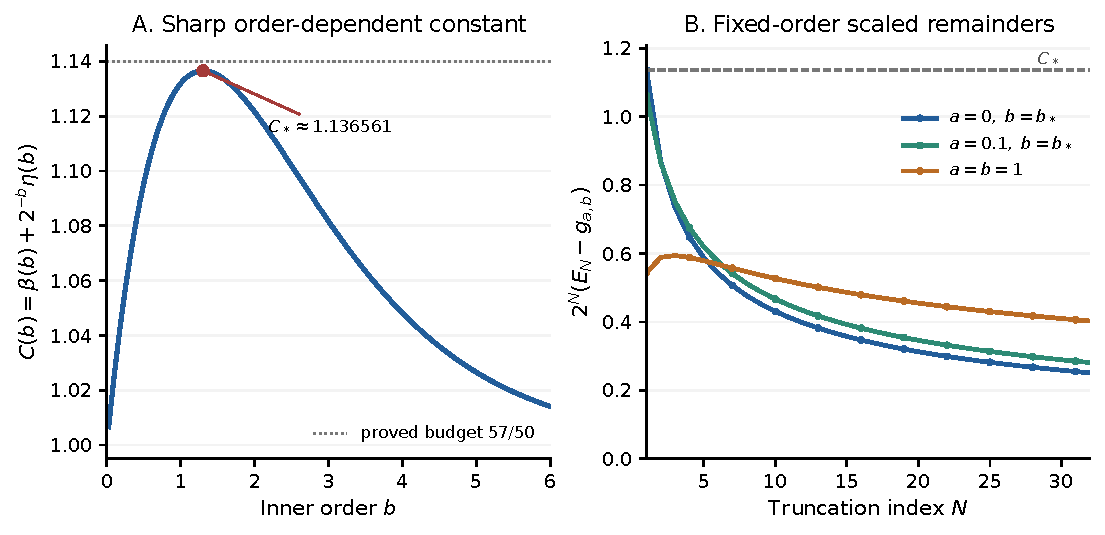
\includegraphics[width=\textwidth]{figures/euler_bounds.pdf}
\caption{Numerical illustrations of the proved Euler bounds.
Panel A shows $C(b)$, its maximum, and the rational budget $57/50$.
Panel B shows fixed-order scaled remainders, including the increase
from $N=1$ to $N=2$ at $a=b=1$. The curve at $a=0$ is the boundary
case allowed by the theorem. The plots illustrate the analytic
proof; the rational global budget is certified separately.}
\label{fig:euler-bounds}
\end{figure}

The constant is specified exactly by \eqref{eq:Cstar}; the decimal
display is not an asserted closed form or a certified enclosure.
The elementary rational constant $5/4$ already follows from the
analytic proof. The following small exact computation improves the
operational constant uniformly over all orders.

\begin{proposition}[A simple rational global budget]\label{prop:rational-budget}
The exact inequalities
\[
 C_*<\frac{5129}{4500}<\frac{57}{50}
\]
hold. Thus $57/50$ is a valid uniform Euler error budget for every
$a\geq0$, $b>0$, and $N\geq1$.
\end{proposition}
\begin{proof}
For $1\leq b\leq2$, gamma differentiation and Cauchy--Schwarz give
\[
 |C'(b)|=|\operatorname{Cov}(\log T_b,\phi(T_b))|
 \leq\sqrt{\psi_1(b)}\,\sqrt{\operatorname{Var}\phi(T_b)}<\frac16.
\]
Indeed $1\leq\phi\leq(1+\sqrt2)/2$ has range less than $1/4$,
so its standard deviation is less than $1/8$. The variance identity
$\operatorname{Var}\log T_b=\psi_1(b)$ follows by differentiating
the gamma integral. Also $\psi_1(b)\leq\psi_1(1)=\pi^2/6<16/9$;
the last inequality follows, for example, from $\pi<22/7$.

The standard-library verifier encloses $C(1+j/30)$ for all
$0\leq j\leq30$ by \eqref{eq:finite-E} with $a=0$, $N=48$,
using a $10^{45}$ grid and integer root inequalities. The already
proved $5/4$ tail bound makes these genuine analytic enclosures.
All thirty-one upper endpoints are strictly less than $1137/1000$.
Every point of $[1,2]$ is within $1/60$ of a node, whence
\[
 C(b)<\frac{1137}{1000}+\frac1{360}=\frac{5129}{4500}
       <\frac{57}{50}.
\]
The proved location $1<b_*<2$ completes the global argument.
Every finite comparison is recorded as a rational inequality in
\src{data/euler_exact_certificate.json}. Neither floating-point
root finding nor a numerical derivative bound enters this proof.
\end{proof}

\begin{remark}[Why the new kernel step is necessary]
At $(a,b)=(1,1)$, the identity
$F_{1,1}(z)=\tfrac12\log^2(1-z)$ gives
$g_{1,1}=-\pi\log2/8$. Therefore
\[
 R_1=\frac{\pi\log2}{4},\qquad
 R_2=\frac{\pi\log2}{2}-\frac12>R_1.
\]
Indeed $\pi>3$ and $\log2>2/3$ imply $\pi\log2>2$.
Thus the scaled errors need not decrease outside the previously
proved right-endpoint region. Bounding $R_N$ by its $N=1$ value
would be invalid even at this simplest integral-order pair.
\end{remark}

\subsection{A general theorem for harmonic sums built from moments}

The argument proves a more general statement that can be reused for
other completely monotone inner sequences. Let $\alpha,\beta$ be
finite positive measures on $[0,1]$, and define
\[
 c_n=\iint t^{n-1}(1+u+\cdots+u^{n-2})\,d\alpha(t)d\beta(u),
 \qquad c_1=0.
\]
Use the definitions \eqref{eq:euler-defs} with $f_n=c_{2n+1}$,
and let $g$ be the imaginary value at $i$ of the continuation
\eqref{eq:F-double}. Difference quotients at $u=1$ are understood
by continuity.

\begin{theorem}[Moment-product Euler principle]\label{thm:moment-general}
For every such pair of measures and every $N\geq1$,
\begin{equation}\label{eq:moment-general}
 0\leq2^N(E_N-g)
 \leq\alpha([0,1])\int_0^1\frac{1+u}{1+u^2}\,d\beta(u)
 \leq\frac{1+\sqrt2}{2}\alpha([0,1])\beta([0,1]).
\end{equation}
The last universal constant is optimal. For probability measures it
is attained at $N=1$, $\alpha=\delta_1$,
$\beta=\delta_{\sqrt2-1}$.
\end{theorem}
\begin{proof}
The finite identities and kernel comparison above remain valid for
arbitrary positive measures. Passing to $u=1$ preserves the inequality
by continuity. The endpoint $t=0$ contributes zero, so it causes no
difficulty. Integrate the pointwise bound, then optimize its last
factor on $[0,1]$. The stated two Dirac masses attain it.
\end{proof}

This theorem identifies the property required for an extension:
the coefficients must be a product of a Hausdorff moment and a finite
partial sum of another moment sequence. It does not assert the same
bound for an arbitrary alternating series or for signed input measures.

\subsection{A certified algorithm and exact identity family}

For every $a\geq0$, $b>0$, the following absolutely convergent identity
is now valid even when the untransformed Gaussian boundary series
fails the term test:
\begin{equation}\label{eq:Euler-identity}
 g_{a,b}=\sum_{j=1}^{\infty}\frac1{2^{j+1}}
       \sum_{n=1}^j(-1)^n\binom jn
           \frac{H_{2n}^{(b)}}{(2n+1)^a}.
\end{equation}
The terms of the outer series are strictly negative, and the first
$N-1$ terms have error bounded by $C(b)2^{-N}$. This is a
proved identity family with an explicit error theorem, rather than
a new name for a formal divergent rearrangement.

The already available finite binomial-tail formula is
\begin{equation}\label{eq:finite-E}
 E_N=2^{-N}\sum_{n=0}^{N-1}(-1)^n
       \frac{H_{2n}^{(b)}}{(2n+1)^a}
                  \sum_{j=n+1}^N\binom Nj.
\end{equation}
The new theorem and Proposition~\ref{prop:rational-budget} supply the
order-independent tail budget $(57/50)2^{-N}$. For rational $a,b$, fractional powers in this finite
sum can be enclosed by integer root inequalities; additions and
multiplications then use rational interval arithmetic. This avoids
the parameter-dependent singular budgets near $a+b=1$ in the earlier
implementation. Given a target absolute radius $\varepsilon$, any
$N$ satisfying $(57/50)2^{-N}\leq\varepsilon$ suffices for the analytic
tail, in addition to the separately controlled finite-sum rounding.

The accompanying program checks this statement using exact rational
arithmetic, including deliberately corrupted candidate controls.
Its numerical comparisons use different representations for selected
known values; a finite check corroborates the analytic proof but does
not replace it. The new global theorem should supplement the more
specialized and sometimes sharper bounds already present in the book.

\subsection{A positive gamma-series identity for the scaled remainder}

The same representation gives an exact identity that exposes the
effect of a large inner order. Let $T,V$ be independent gamma
variables of rate one and respective shapes $a,b$; for $a=0$
take $T=0$ deterministically. Define
\[
 J_N(s)=\mathbb E\bigl[W_N(e^{-2Y_s})\bigr],
 \qquad Y_s\sim\operatorname{Gamma}(s,1),
 \qquad J_N(0)=W_N(1)=0.
\]
In particular, for $s>0$ this is the positive integral
\[
 J_N(s)=\frac1{\Gamma(s)}
 \int_0^\infty y^{s-1}e^{-y}
             \frac{(1-e^{-2y})^N}{1+e^{-2y}}\,dy.
\]

\begin{proposition}[Positive gamma-series identity]
\label{prop:gamma-remainder-series}
For all $a\geq0$, $b>0$ and integers $N\geq1$,
\begin{equation}\label{eq:gamma-remainder-series}
 R_N(a,b)=\sum_{r=1}^{\infty}r^{-b}
  \mathbb E\left[
   W_N\bigl(e^{-2(T+V/r)}\bigr)-W_N(e^{-2T})\right].
\end{equation}
Every summand is nonnegative, and the series converges.
If $b>1$, its first term gives the uniform enclosure
\begin{equation}\label{eq:gamma-remainder-first}
 0\le R_N(a,b)-\{J_N(a+b)-J_N(a)\}\le\zeta(b)-1.
\end{equation}
\end{proposition}
\begin{proof}
In logarithmic coordinates the exact two-measure formula reads
\[
 R_N(a,b)=\mathbb E
 \frac{W_N(e^{-2(T+U)})-W_N(e^{-2T})}{1-e^{-U}},
 \qquad U\sim\operatorname{Gamma}(b,1),
\]
with $T,U$ independent. Expand $(1-e^{-U})^{-1}$ as a
positive geometric series. Tonelli's theorem applies because
the numerator is nonnegative. Multiplying the rate-one gamma
density of $U$ by $e^{-(r-1)U}$ produces $r^{-b}$ times
the density of $V/r$. This proves
\eqref{eq:gamma-remainder-series}; its convergence follows
from Theorem~\ref{thm:Euler-uniform}.
The sum of independent rate-one gamma variables has the
sum of their shapes, so the $r=1$ term is
$J_N(a+b)-J_N(a)$. Every other expectation lies in $[0,1]$,
which proves \eqref{eq:gamma-remainder-first}.
\end{proof}

The enclosure is independent of $a$ and $N$. For large $b$,
it replaces a two-variable integral by a difference of two
positive one-variable integrals with an exponentially small
budget in $b$. For $b\leq1$ the positive series identity
still holds, but the crude tail estimate by $\zeta(b)-1$
must not be used.

\subsection{Logarithmically growing orders: a phase law for Euler errors}

The fixed-order statement $R_N\to0$ cannot be made uniform
over all positive orders. The following theorem identifies
an explicit transition and its two boundary profiles.
Write
\[
 \Phi_{\mathrm G}(x)=\frac1{\sqrt{2\pi}}
                    \int_{-\infty}^x e^{-y^2/2}\,dy
\]
for the standard normal distribution function.

\begin{theorem}[Moving-order Euler phase law]
\label{thm:euler-moving}
Let $\ell=\log N$. Suppose
\[
 a_N=A\ell+\alpha\sqrt{\ell}+o(\sqrt{\ell}),\qquad
 b_N=B\ell+\beta\sqrt{\ell}+o(\sqrt{\ell}),
 \qquad A,B>0,
\]
where $\alpha,\beta$ are fixed real numbers. Then
\begin{equation}\label{eq:euler-phase}
 R_N(a_N,b_N)\longrightarrow
 \begin{cases}
  0,& A+B<1/2,\\
  \Phi_{\mathrm G}(\sqrt2(\alpha+\beta)),&A+B=1/2,\\
  1,&A<1/2<A+B,\\
  \Phi_{\mathrm G}(-\sqrt2\alpha),&A=1/2,\\
  0,&A>1/2.
 \end{cases}
\end{equation}
The cases are disjoint because $B>0$, and cover the stated
parameter range. In particular,
\[
 \liminf_{N\to\infty}\ \sup_{a,b>0}R_N(a,b)\geq1.
\]
\end{theorem}
\begin{proof}
Since $b_N\to\infty$, \eqref{eq:gamma-remainder-first}
shows that
\[
 R_N(a_N,b_N)=J_N(a_N+b_N)-J_N(a_N)+o(1).
\]
For example $\zeta(b)-1\leq2^{-b}+2^{1-b}/(b-1)$ for
$b>1$, by an integral comparison, so the discarded term
tends to zero. It remains to evaluate $J_N(s_N)$ for
\[
 s_N=c\ell+\gamma\sqrt{\ell}+o(\sqrt{\ell}),\qquad c>0.
\]

The function $W_N(e^{-2y})$ is an approximate threshold at
$y=\ell/2$. Set $h_N=\ell^{1/4}$. If
$y\leq\ell/2-h_N$, then
\[
 0\leq W_N(e^{-2y})\leq\exp(-e^{2h_N}).
\]
If $y\geq\ell/2+h_N$, Bernoulli's inequality gives
\[
 0\leq1-W_N(e^{-2y})
 \leq(N+1)e^{-2y}\leq2e^{-2h_N}.
\]
Thus the expectation of its difference from
$\mathbf1_{\{Y_{s_N}>\ell/2\}}$ tends to zero provided
\[
 \mathbb P\bigl(|Y_{s_N}-\ell/2|\leq h_N\bigr)\to0.
\]
When $c\ne1/2$, this follows from
$Y_{s_N}/\ell\to c$ in probability, since
$\operatorname{Var}Y_{s_N}=s_N=O(\ell)$.
When $c=1/2$, it follows from the gamma central limit
theorem and $h_N/\sqrt{s_N}\to0$.
For completeness, that central limit theorem follows
directly from the characteristic function
\[
 \mathbb E e^{it(Y_s-s)/\sqrt{s}}
 =e^{-it\sqrt{s}}(1-it/\sqrt{s})^{-s}
 \longrightarrow e^{-t^2/2}.
\]
The limiting normal distribution is continuous, so intervals
whose standardized widths tend to zero have probability
tending to zero, including at the moving centers here.

Consequently
\[
 J_N(s_N)\longrightarrow
 \begin{cases}
 0,&c<1/2,\\
 \Phi_{\mathrm G}(\sqrt2\gamma),&c=1/2,\\
 1,&c>1/2.
 \end{cases}
\]
Apply this first to $s_N=a_N+b_N$ and then to $s_N=a_N$.
Their difference gives all five cases in
\eqref{eq:euler-phase}, using
$1-\Phi_{\mathrm G}(x)=\Phi_{\mathrm G}(-x)$.
Choosing, for example, $A=B=1/3$ proves the final assertion.
\end{proof}

The phase law supplies the lower bound in an asymptotically
sharp global result.

\begin{theorem}[Asymptotically optimal global constant]
\label{thm:euler-asymptotic-budget}
Let
\[
 C_N=\sup_{a,b>0}2^N(E_N(a,b)-g_{a,b}).
\]
Then
\begin{equation}\label{eq:CN-limit}
 \lim_{N\to\infty}C_N=1.
\end{equation}
The same conclusion holds if $a=0$ is included in the supremum.
\end{theorem}
\begin{proof}
Put $F_N(y)=W_N(e^{-2y})$. This function is increasing from
zero to one and satisfies $0\leq F_N'(y)\leq4$ uniformly in
$N\geq1$, $y\geq0$. Indeed, with $x=e^{-2y}$,
\[
 F_N'(y)=
 \frac{2x(1-x)^{N-1}\{N+1+(N-1)x\}}{(1+x)^2}.
\]
For $N\geq2$ it is at most
$4Nx(1-x)^{N-1}\leq4$; for $N=1$ it is at most one.
For every finite $L$, $\sup_{0\leq y\leq L}F_N'(y)\to0$.

Let $M(a)$ be the maximum of the density of
$\operatorname{Gamma}(a,1)$ for $a>1$. Conditional on $U=u$,
positivity of $F_N'$ and $\int_0^\infty F_N'=1$ give
\[
 \mathbb E_T[F_N(T+u)-F_N(T)]
 =\int_0^u\mathbb E_T F_N'(T+s)\,ds
 \leq uM(a).
\]
Since $u/(1-e^{-u})\leq1+u$ for $u\geq0$, it follows that
\begin{equation}\label{eq:large-a-bound}
 R_N(a,b)\leq M(a)(1+b).
\end{equation}
Moreover $M(a)\to0$ as $a\to\infty$. An elementary quantitative
bound suffices: for $L=a-1\geq4$, the gamma density has its
maximum at $L$, and on $|y-L|\leq\sqrt L/2$,
\[
 \log\frac{p_a(y)}{p_a(L)}
 =L\log\left(1+\frac{y-L}{L}\right)-(y-L)\geq-\frac14,
\]
using $\log(1+z)\geq z-z^2$ for $|z|\leq1/2$.
Integrating on that interval yields
$M(a)\leq e^{1/4}/\sqrt{a-1}$.

We also need uniform convergence on bounded order rectangles:
\begin{equation}\label{eq:compact-order-zero}
 \sup_{0\leq a\leq A_0,\ 0<b\leq B_0}R_N(a,b)\longrightarrow0
 \qquad(A_0,B_0<\infty).
\end{equation}
For any fixed pair in the rectangle, couple independent gamma
variables so that $T\leq T_0$ and $U\leq U_0$, where
$T_0,U_0$ have shapes $A_0,B_0$ and rate one. The gamma
addition rule supplies this coupling; shape zero is a point
mass at zero. The exact kernel is bounded by
\[
 \frac{F_N(T+U)-F_N(T)}{1-e^{-U}}
 \leq(1+U_0)\sup_{0\leq y\leq T_0+U_0}F_N'(y).
\]
The last random variable is independent of the smaller
orders, is bounded by $4(1+U_0)$, and tends to zero almost
surely. Dominated convergence proves
\eqref{eq:compact-order-zero}.

Now fix $\varepsilon>0$. Choose $B_0>1$ so large that
$\zeta(B_0)<1+\varepsilon$. For $b>B_0$,
\eqref{eq:gamma-remainder-first} gives
$R_N(a,b)\leq\zeta(b)<1+\varepsilon$, uniformly in $a,N$.
For $b\leq B_0$, choose $A_0$ sufficiently large that
\eqref{eq:large-a-bound} is less than $\varepsilon$
for all $a>A_0$. The remaining compact rectangle is
controlled by \eqref{eq:compact-order-zero}. Thus
$\limsup C_N\leq1+\varepsilon$. Let $\varepsilon\downarrow0$.
The choice $a_N=b_N=(\log N)/3$ in
Theorem~\ref{thm:euler-moving} gives $\liminf C_N\geq1$.
This proves \eqref{eq:CN-limit}, also with the axis included.
\end{proof}

The global constant $C_*>1$ and the asymptotic constant one
answer different questions. The first is sharp uniformly
over all truncation indices; the second is the limit of
the optimal order-uniform constant at index $N$.
The proof of the latter does not give an effective rate for
$C_N-1$, nor does it assert that $C_N$ decreases in $N$.

\subsection{An explicit lower asymptotic for the optimal constant}
\label{sec:axis-asymptotic-budget}

For the scaled Euler remainder $R_N(a,b)=2^N(E_N-g_{a,b})$, write
$C_N=\sup_{a,b>0}R_N(a,b)$. Values at $a=0$ give lower bounds for
this supremum by continuity as $a\downarrow0$. The positive integral
representation gives
\[
 R_N(0,b)=\int_0^1 K_N(u)\,d\sigma_b(u),\qquad
 K_N(u)=\frac{(1+u)(1-u^2)^{N-1}}{1+u^2}.
\]

\begin{proposition}[Explicit axis asymptotics]
\label{prop:euler-axis-lower}
Put
\[
 p=\frac{\log2}{\log(3/2)},\qquad
 q=\frac{\log3}{\log2},\qquad
 c=(1-q^{-1})q^{-p},\qquad
 \widehat b_N=\frac{\log(Nq)}{\log(3/2)}.
\]
For every integer $N\ge1$ and $b>0$,
\begin{align*}
 R_N(0,b)&=1+2^{-b}-N3^{-b}-N4^{-b}+\varepsilon_N(b),\\
 0&\le\varepsilon_N(b)\le
       \frac{N^2-N+2}{2}\bigl(5^{-b}+6^{-b}\bigr).
\end{align*}
Consequently,
\[
 R_N(0,\widehat b_N)=1+cN^{-p}+o(N^{-p}),\qquad
 \liminf_{N\to\infty}N^p(C_N-1)\ge c.
\]
\end{proposition}

\begin{proof}
Let $F_N(s)=(1-s)^{N-1}/(1+s)$. Then
$F_N(0)=1$, $F_N'(0)=-N$, and
$0\le F_N''(s)\le N^2-N+2$ on $[0,1]$.
For $N\ge3$ the last assertion follows term by term from
\begin{align*}
 F_N''(s)={}&
 \frac{(N-1)(N-2)(1-s)^{N-3}}{1+s}
 +\frac{2(N-1)(1-s)^{N-2}}{(1+s)^2}
 +\frac{2(1-s)^{N-1}}{(1+s)^3}.
\end{align*}
For $N=1,2$ it follows directly from
$F_1(s)=(1+s)^{-1}$ and $F_2(s)=2(1+s)^{-1}-1$.
Taylor's integral remainder therefore gives
\[
 0\le F_N(s)-1+Ns\le\frac{N^2-N+2}{2}s^2.
\]
Multiply by $1+u$, set $s=u^2$, and use
$\int u^j\,d\sigma_b(u)=(j+1)^{-b}$. This proves the explicit
remainder bounds.

The function $2^{-b}-N3^{-b}$ has its unique maximum at
$b=\widehat b_N$, where its value is $cN^{-p}$. At that value of $b$,
the omitted terms are bounded in magnitude by
\[
 O\!\left(N^{1-2p}
       +N^{2-\log5/\log(3/2)}\right)=o(N^{-p}).
\]
Indeed $p>1$, and
$\log5/\log(3/2)>p+2$ is equivalent to $5>9/2$.
This proves the asymptotic identity and the lower bound for $C_N$.
\end{proof}


Numerically, $p=1.70951129135145477698\ldots$ and
$c=0.16794779654251279566\ldots$. The lower bound is a theorem;
the matching upper asymptotic over all positive orders is
the separate conjecture in Section~\ref{sec:research}.
